\documentclass[14pt,a4paper]{book}

% Използване на български език.
\usepackage[english,bulgarian]{babel}
\usepackage[utf8]{inputenc}

% Използване на графика.
\usepackage[pdftex]{graphicx}

% Използване на PDF-и за кориците.
\usepackage{pdfpages}

% Използване на хедър и футър.
\usepackage{fancyhdr}

% Използване на кавички при цитиране.
\usepackage{dirtytalk}

% Използва се за създаване на азбучен указател.
\usepackage{imakeidx}

% Използва се за сензитивни хипер-връзки в самия документ.
\usepackage[pdftex, bookmarks, linktocpage]{hyperref}

% Заглавие.
\title{Блоково програмиране със Scratch и App Inventor}

% Автори.
\author{Тодор Балабанов, Галя Петрова}

% Директория с изображения.
\graphicspath{{images/}}

% Избор на активен език.
\selectlanguage{bulgarian}

% Текстове за декорация на страницата в горната и долната част.
\pagestyle{fancy}
\fancyhf{}
\fancyhead[LE,RO]{\thepage}
\fancyhead[RE]{Блоково програмиране със Scratch и App Inventor}
\fancyhead[LO]{Тодор Балабанов, Галя Петрова}
\fancyfoot[LE,RO]{Издателство \say{Образование и Познание}, 2020}

% Дебелина на разделителната линия.
\renewcommand{\headrulewidth}{2pt}
\renewcommand{\footrulewidth}{1pt}

% Генериране на азбучен указател.
\onecolumn
\makeindex[columns=2, title=Азбучен указател, intoc]

% Начало на документа.
\begin{document}

% Предна корица.
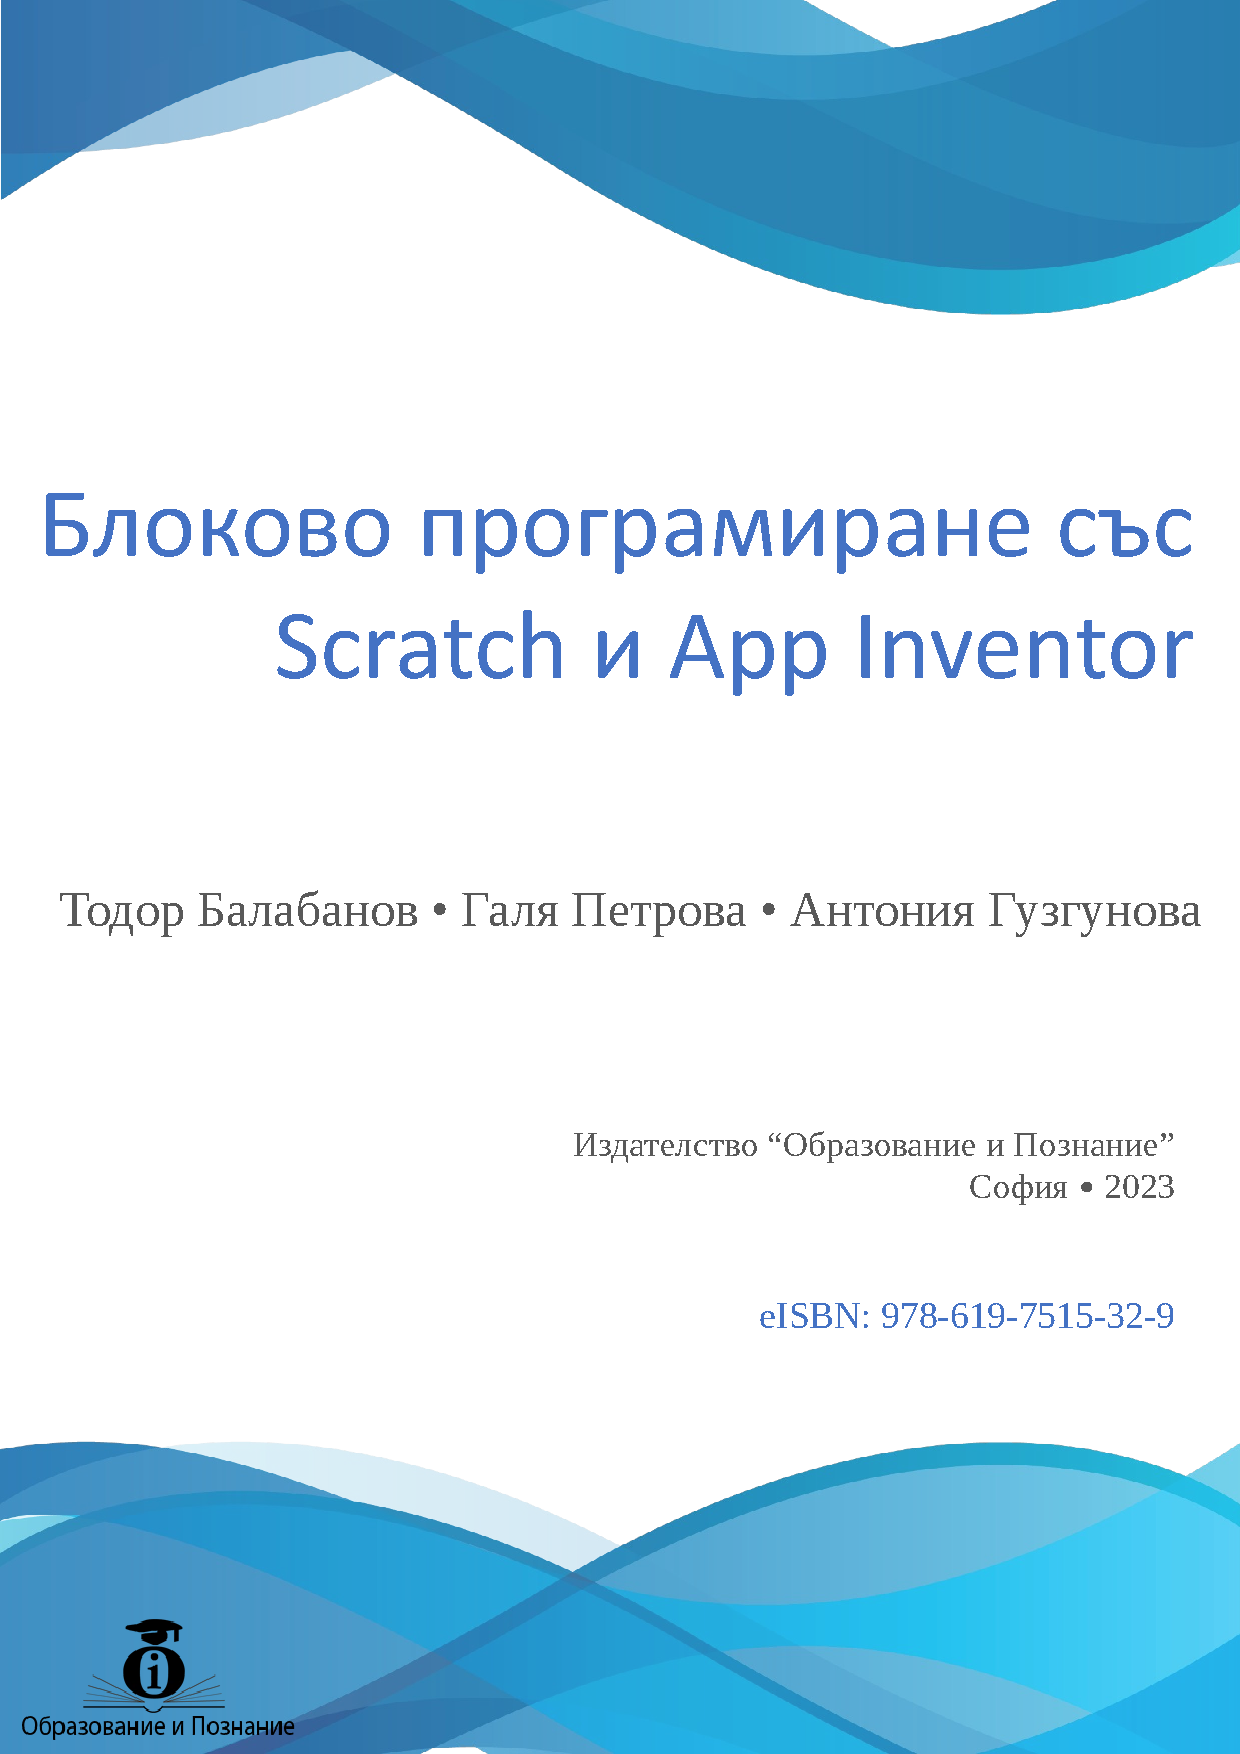
\includepdf[pages={1}]{covers/front}
\thispagestyle{empty}

% Страница с авторски права.
~\vfill
\thispagestyle{empty}

\noindent Авторски права \copyright\ 2022 \\

\noindent Тодор Балабанов, Галя Петрова \\ 

\noindent \textsc{Издателство \say{Образование и Познание}} \\
\noindent \textsc{https://www.obrazovaniebg.net/} \\

\noindent Разпространява се под свободен лиценз: \\ 
Creative Commons Attribution-NonCommercial-NoDerivatives 4.0 \\
International Public License \\
\url{https://creativecommons.org/licenses/by-nc-nd/4.0} \\

\noindent {\footnotesize This book was partially supported by the Bulgarian National Science Fund by the project \say{Mathematical models, methods and algorithms for solving hard optimization problems to achieve high security in communications and better economic sustainability, KP-06-N52/7/19-11-2021}}. \\

\noindent \textit{Първо издание, 2022}

% Таблица на съдържанието.
\thispagestyle{empty}
\pagestyle{empty}
\tableofcontents
\thispagestyle{empty}
\pagestyle{empty}

% Отделните глави са в отделни файлове.
\newpage
\pagestyle{fancy}
\pagenumbering{arabic}
\setcounter{page}{1}
\addcontentsline{toc}{chapter}{Предговор}
\chapter*{Предговор}
\thispagestyle{empty}

Тази книга е предназначена за всички хора, които се вълнуват от теми в програмирането и най-вече за обучението на деца в тази област. Надеждата ни е, че всеки с интерес в областта би намерил нещо ценно в изложения материал. Нашият опит е предимно свързан с академичния свят и педагогиката, посветена на обучението на деца. Материалът е изложен по такъв начин, че да разкрива основните механизми за учене чрез правене. Най-общо казано, книгата съпровожда читателя с минимални компютърни познания до едно задоволително ниво на разбиране за концепциите в програмирането. 

От наша гледна точка, представянето на програмните конструкции с помощта на визуализация, максимално доближаваща класическите пъзели, дава широки възможности за усвояване на ценни знания и умения. Подобен подход за онагледяване позволява ефективно снижаване на възрастта за обучение по програмиране. Докато класическите програмни езици са подходящи в класовете на гимназията, блоковите езици ефективно намират своето приложение в прогимназиалния курс на обучение. 

Част от изложения материал разяснява фундаментални концепции в програмирането, като - последователност от инструкции, условни и безусловни преходи, цикличност на действията, събития, модулна организация и други. Друга част набляга на практическа реализация и то на идеи, които имат потенциал да се превърнат в самостоятелни софтуерни решения. Избраният подход за представяне на информацията е чрез примери на принципа – направа, стъпка по стъпка. 

Книгата не предполага предварителни изисквания за напреднало ниво на компютърна грамотност, но разчита читателят да има базови познания за това какво е компютърна система, какво е операционна система, какво е Интернет, как се борави със зареждането и преглеждането на уеб страници. Разгледаните системи за блоково програмиране са уеб базирани и работата с тях се осъществява в облачно пространство. Не се изискват задълбочени познания по математика, но за разбирането на някои от примерите много помагат базови познания по алгебра и геометрия. Артистични умения, като музикалност или изобразителни изкуства не са нужни, но наличието им би дало допълнителен колорит на постигнатите резултати. 

Материалът е организиран в глави, които са свързани една с друга и за по-пълноценно усвояване е желателно прочитането им да се извърши в зададената последователност. Част от изложението в книгата се базира на учебни предмети, преподавани в прогимназиалния курс на обучение.

\vspace{0.5cm}

\large{\textbf{Благодарности}}

\vspace{0.5cm}

Авторите биха искали да благодарят на своите семейства за търпението и разбирането, проявено в дългият период за написването на тази книга. Също така биха искали да благодарят на своите колеги и приятели, помогнали в достигането на едно по-високо качество. 




\newpage
\addcontentsline{toc}{chapter}{Заключение}
\chapter*{Заключение}
\thispagestyle{empty}

Блоковото програмиране е ефективен и достъпен начин за запознаване на децата с концепциите за кодиране. Чрез разбиването на програмирането на визуални блокове, децата могат да се научат да сглобяват малки програми, без да се притесняват за синтаксис или грешки при въвеждане. Програмните среди Scratch и App Inventor са доказал се в практиката инструменти за преподаване на блоково програмиране на деца. Интуитивният интерфейс и цветните блокове на Scratch го правят идеален вариант за по-малки деца, докато способността на App Inventor да създава реални мобилни приложения може да се хареса на по-големите. Книгата предоставя изчерпателно ръководство за изучаване на блоково програмиране със Scratch и App Inventor. Обхваща проектиране и създаване на игри, създаване на мобилни приложения и други. Книгата също така включва инструкции стъпка по стъпка и много визуални примери, които да помогнат на децата да разберат концепциите за програмиране. Децата могат да развият основни умения като решаване на проблеми, логическо мислене и креативност чрез блоково програмиране. Тези умения могат да бъдат приложени в бъдещи начинания, включително компютърни науки и други области от науката, технологиите, инженерството и математиката. Като цяло, книгата за блоково програмиране за деца със Scratch и App Inventor е отличен ресурс за родители и преподаватели, които искат да запознаят децата с възможностите на програмирането. Използвайки визуални блокове и лесни за разбиране инструкции, децата могат да се научат да кодират по забавен и увлекателен начин, което ги подготвя за бъдещ успех в личен и професионален план.



% Списък с използвана литература и източници на информация.
\newpage
\begin{thebibliography}{99}
\addcontentsline{toc}{chapter}{Библиография}
\end{thebibliography}

% Азбучен указател на използваните термини.
\newpage
\printindex

% Задна корица.
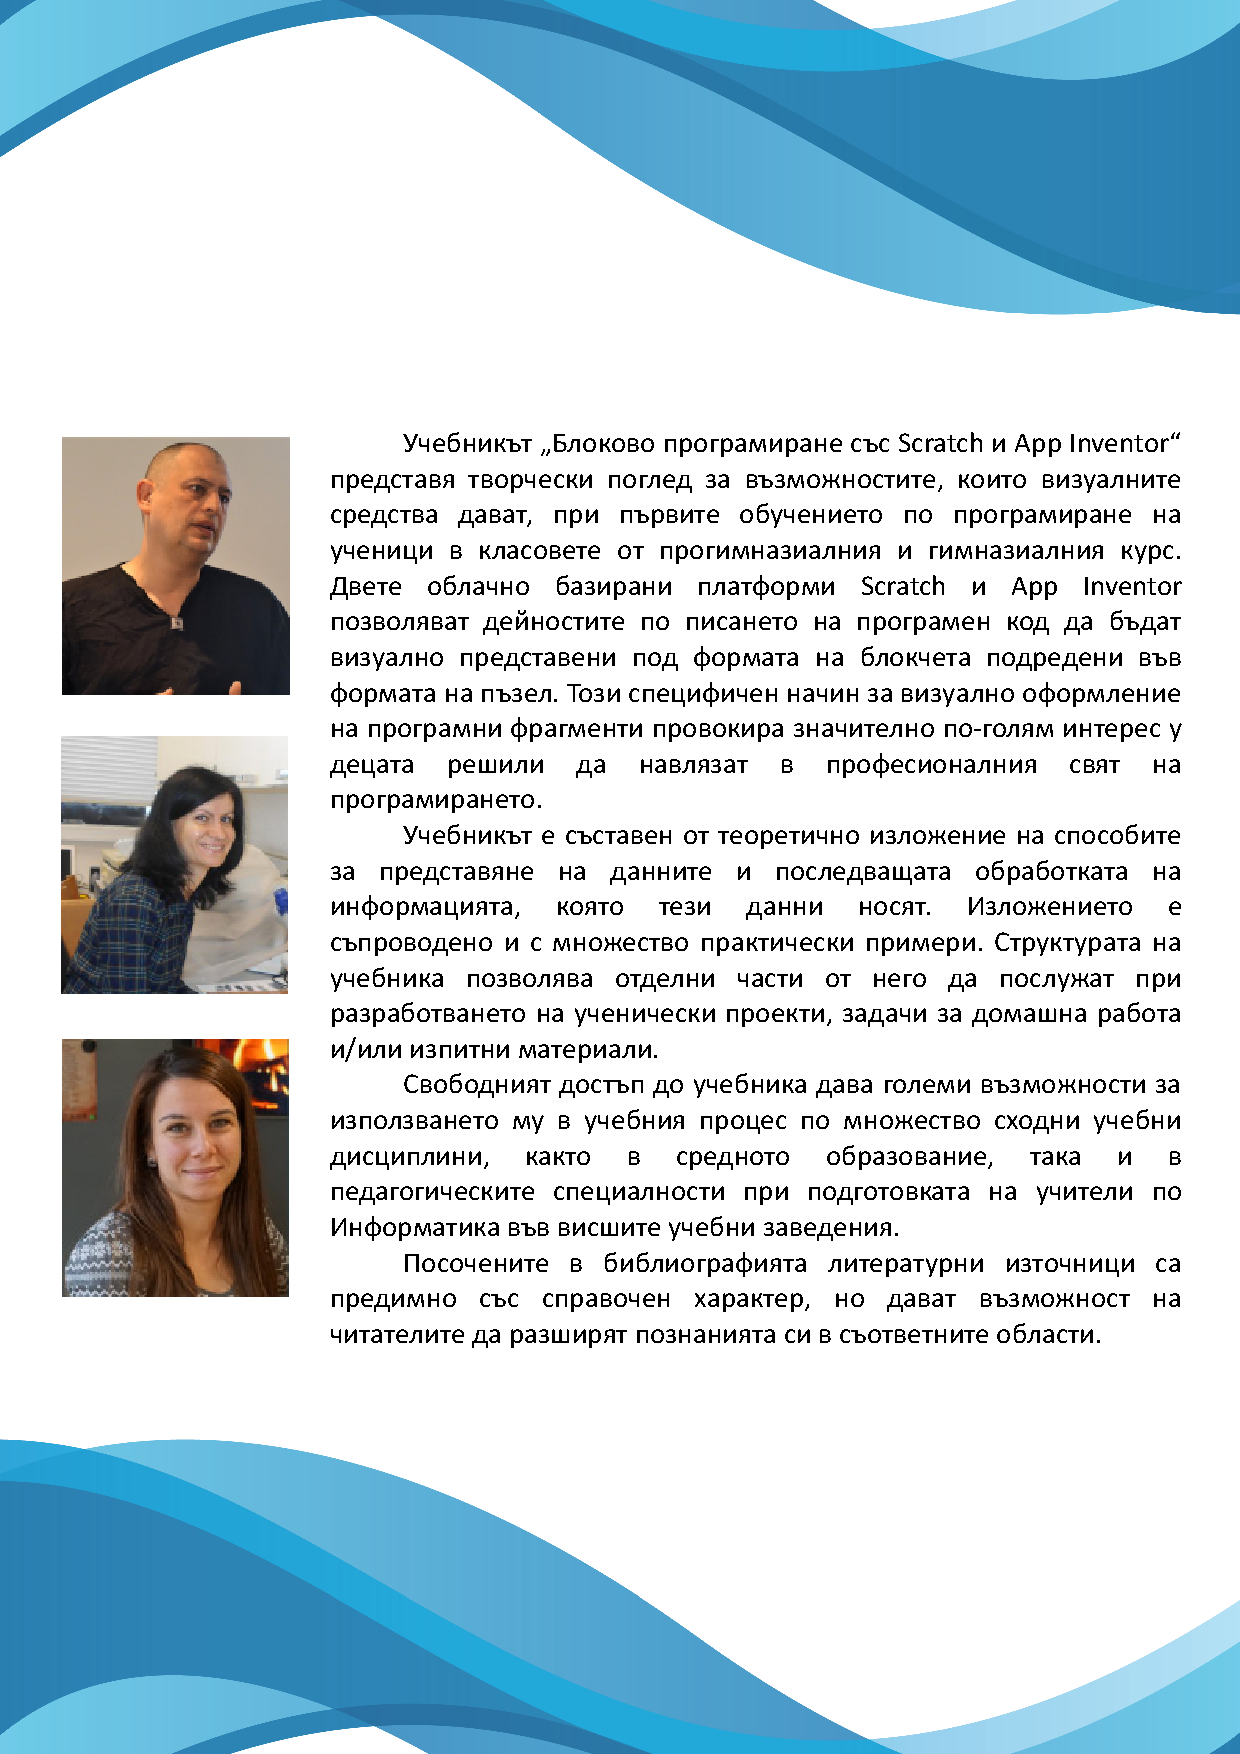
\includepdf[pages=-]{covers/back}

\end{document}
